\section{Methods}
\label{Methods}
% This should be fairly brief, the system is not particularly complex.
For the SORA flights, a MiniPIX with a USB interface was coupled with a low cost open ARM based computer called Raspberry Pi 3.  Both flights utilized a Raspberry Pi 3 to communicate and handle all operations with the MiniPIX.  This system allowed for remote operation and on-board analyzation of all data.  The SORA flights tested the feasibility of these low-cost systems to fly further upper atmospheric and near-space missions.  

The PyPixet library, developed by Daniel Turcek (CITE ME), controlled the MiniPIX device used in both SORA flights.  The 2017 flight was the first testbed for MiniPIX setup, testing the limits of the hardware and software setup.  The 2018 flight was more robust and applied many improvements based on challenges faced during the initial flight.  Important changes included support for an arbitrary number of MiniPIX detectors to record data simultaneously.  Furthermore, the 2018 flight software allowed for direct serial uplink and downlink. This supported observation of real-time data, adjusting the MiniPIX's shutter rate, and controlling the acquisition settings.

\subsection{Configuration and Calibration}
% Device parameters, threshold, bias voltage, shutter time etc.
\subsection{System Design}
% RPI interface to MiniPIX, heatsink design etc.
Additive manufacturing was utilized to create a custom made case for the MiniPIX device.  As seen in Figure ~\ref{fig:minipix_case}, the MiniPIX case is in white, while the heat sink setup is in blue-gray color (COME AND FIX ME).  In the early vacuum tests, it was found that the MiniPIX would require a passive cooling method to keep the device at operational levels.  At the same time, the ABS plastic enclosure acted as insulation, maintaining the MiniPIX temperatures in stable ranges.  The MiniPIX device was mated to the heatsink via a bracket (not shown in the figure ~\ref{fig:minipix_case}) and with thermal adhesive.
\begin{figure}[h]
    \centering
    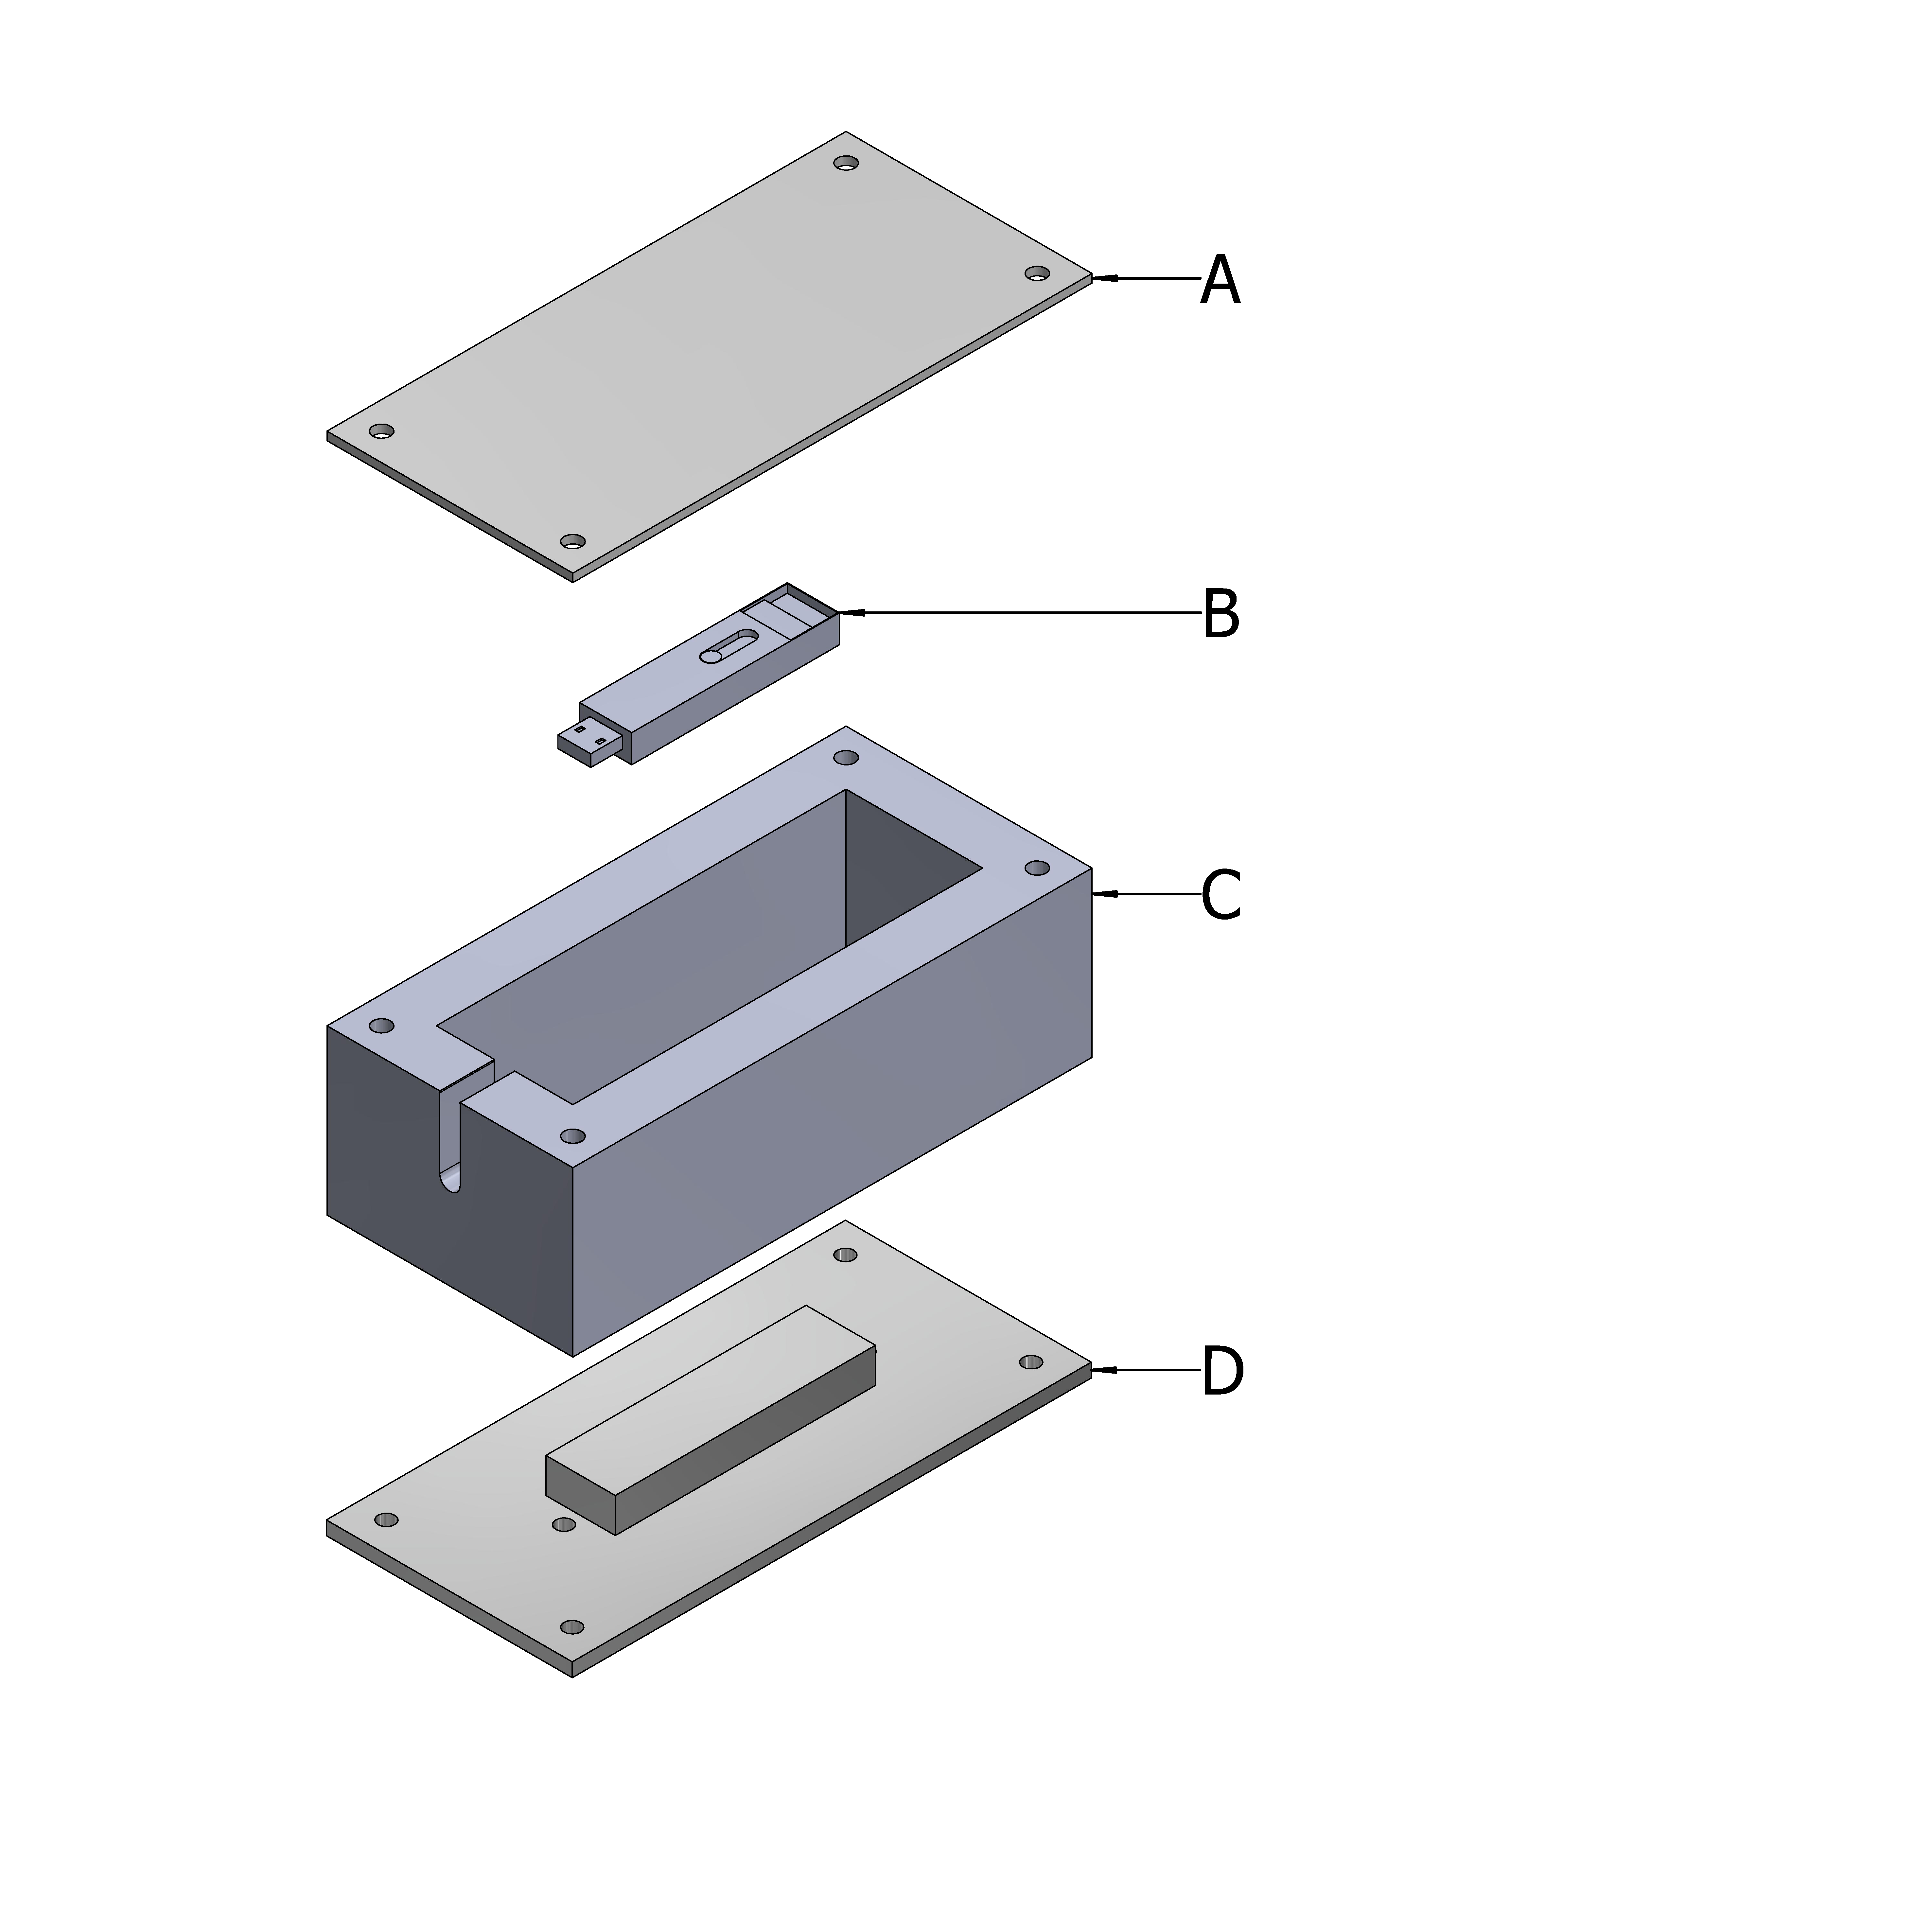
\includegraphics[width=0.25\textwidth]{Minipix_case_assembly.pdf}
    \caption{MiniPIX Case Assembly}
    \label{fig:minipix_case}
\end{figure}
The MiniPIX case allowed for a USB cable to be routed through the enclosure to interface directly to the Raspberry Pi.  This allowed the MiniPIX device to be modular and be place in different configurations for both flights.  The Raspberry Pi was placed in a separate location within the payloads near the power supply.  Overall, the payload was modular and accessible.



